\section{Rosemary Design}
\label{reuse-rosemary}

The overall workings of Rosemary have been described in the previous section.
Below the architecture and data model will be explained before going into the implementation as done in the \ivfsystem{}, which will be described in the next section.

\begin{figure}[!hb]
	\centering
	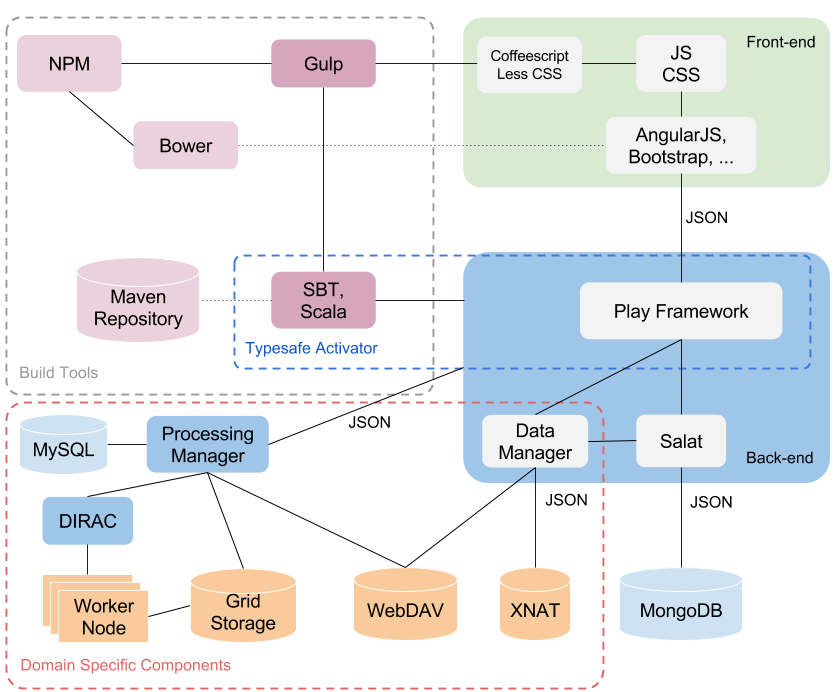
\includegraphics[width=0.7\linewidth]{images/rosemary-architecture}
	\caption{
		Rosemary architecture with domain specific items removed.
		Describes the implementation of the back-end and the front-end.
		Together with the specific build tools used during development.
	}
	\label{fig:reuse-rosemary-architecture}
\end{figure}

\paragraph{Architecture}
For the Rosemary back-end the Play Framework \cite{play} is used.
It is written with the Scala \cite{scala} programming language which is interoperable with Java.
As a database mongoDB \cite{mongo} is used, a document-oriented database.
Communication between the back-end and the database is done with JSON \cite{json} and the Scala library `Salat' is used to serialise the JSON information into Scala classes.
The back-end exposes a RESTful API which can be accessed by the front-end.

The front-end is based on the AngularJS \cite{angular} framework and coded with Coffeescript \cite{coffeescript} which is compiled into JavaScript.
For layout and styling HTML and Less \cite{less} are used, Less compiles into CSS.
To provide a pleasant user experience the front-end is developed as a web application, data is loaded asynchronous through the RESTful API and stored at the client's side to give the feel of a native application.

%\begin{figure}[!hb] 
%	\centering
%	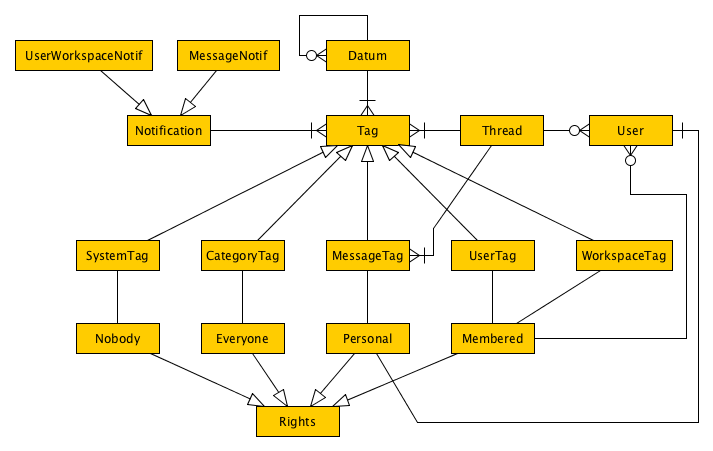
\includegraphics[width=1.0\linewidth]{images/datamodel-clean}
%	\caption{
%		Rosemary data model with domain specific items removed.
%		Describes the workspace, tagging, datum, and notification models.
%		The unedited Rosemary data model can be found in appendix \ref{unedited-datamodel}.
%	}
%	\label{fig:reuse-rosemary-dm}
%\end{figure}

\paragraph{Data model}
The yellow components in figure \ref{fig:implementation-rosemary-dm} depict the Rosemary data model with the domain specific items removed.
The model contains six main data objects: {\tt Datum}, {\tt Tag}, {\tt Rights}, {\tt User}, {\tt Notification}, and {\tt Thread}.
The {\tt Tag}, {\tt Notification}, and {\tt Rights} objects are inherited to describe a specific instance, for example {\tt WorkspaceTag} is a kind of {\tt Tag}.

A short description of the main objects will be given for better understanding of the model.
A {\tt Datum} is a single piece of data and its metadata, for the Rosemary case a {\tt Datum} might be a reference to an MRI image and metadata about the scanned patient.
{\tt Datum}s may be tagged with the {\tt Tag} object, for example, the {\tt UserTag} is a tag defined by the user and attached to a set of {\tt Datum}s for identification.
{\tt Tag}s are also used to manage access rights, each tag has a specific {\tt Rights} attached to it.
Based on the set of {\tt User}s which is assigned to the {\tt Rights} the system can restrict access to certain data.
The {\tt Notification} object stores data about process milestones which can be displayed in the user interface, for example when a message is send.
Lastly, the {\tt Thread} keeps track of messages send back and forth in conversations.

The data model and its implementation provide some interesting possibilities.
For example, a {\tt Datum} can be tracked and reused endlessly by applying a {\tt Tag} object.
One use of this is access control, which can be applied by tagging a {\tt Datum} with a {\tt WorkspaceTag} which is owned by a {\tt User}.
Many different constructs of this sort can be achieved without ever touching the structure of the actual model itself.
%The reuse in the \ivfsystem{} relies heavily on this concept, which means only slight changed had to be made to the original data objects.